\chapter{Vulnerabilities exploitation on the bus: wishbone, AXI-Lite et AXI}
Building on the previously established experimental setup, this chapter investigates the vulnerabilities of three widely used SoC bus protocols—Wishbone, AXI-Lite, and AXI—under fault injection attacks. These interconnects play a central role in processor-memory communication and are potential points of failure when exposed to transient faults. We briefly introduce each protocol's relevant features, followed by targeted fault injection experiments designed to assess their resilience. By comparing their behavior under similar fault scenarios, we identify protocol-specific weaknesses and extract general insights into bus-level fault tolerance.
\section{Introduction of bus}

\subsection{Wishbone}
We conducted an in-depth examination of each signal within the Wishbone bus, referencing their definitions from the official Wishbone specification. By analyzing the Verilog source code, inspecting Vivado’s elaborated design, and consulting publicly available diagrams~\cite{wishbonewiki}, we assembled a modular SoC architecture that explicitly delineates the Wishbone interconnect and its peripheral components.

The overall structure is depicted in Figure~\ref{architecturebus}. Data transmission is handled by \texttt{DAT\_I} (data input) and \texttt{DAT\_O} (data output), enabling bidirectional communication between the processor and memory modules. Address targeting is managed via \texttt{ADR\_O}, which designates the intended memory address. Control signals include \texttt{WE\_O} (write enable) to indicate write cycles, \texttt{STB\_O} (strobe) to signal valid operations, and \texttt{CYC\_O} (cycle) to initiate active bus phases. Handshaking is achieved through \texttt{ACK\_I} (acknowledge signal), which validates the completion of a data transaction. Byte-level data access is supported by \texttt{SEL\_O} (byte select). Additionally, \texttt{CLK\_I} supplies the system clock, while \texttt{RST\_I} resets the bus interface for proper startup. Certain extended implementations also incorporate \texttt{TAGN\_O} and \texttt{TAGN\_I}, used to convey auxiliary metadata for advanced bus operations.

\begin{figure}[t!]
  \centering
  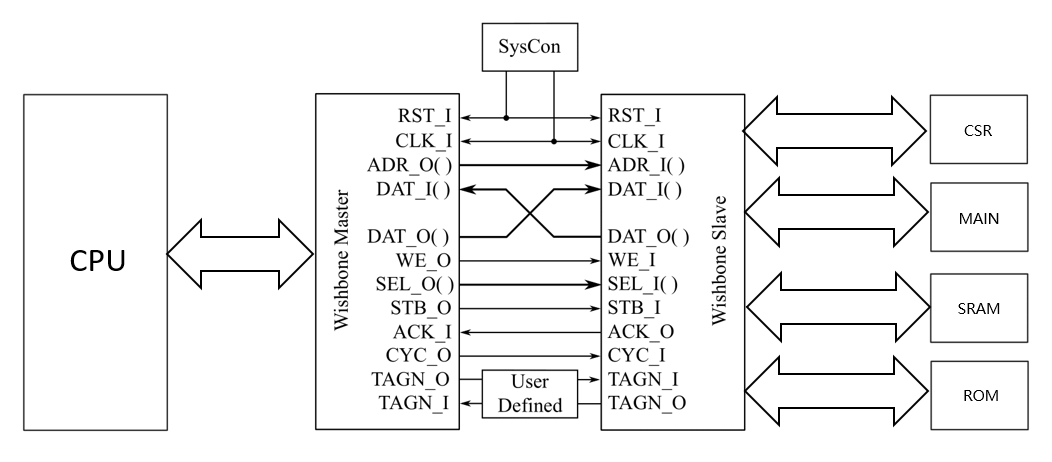
\includegraphics[width=\linewidth]{Chapitre3/figures/Wishbone.png}
  \caption{Signals exchange between CPU and memory via Wishbone bus}
  \label{architecturebus}
\end{figure}

Data transfer operations rely on the configuration of control registers. Here, we highlight two of the most critical: \texttt{SEL} and \texttt{ACK}.

The \texttt{SEL} register (Figure~\ref{sel}) is a 4-bit selector, with each bit corresponding to one of four memory blocks. It functions as a memory selection indicator, specifying which memory module the CPU interacts with during data access. The \texttt{SEL} value is derived from the address register \texttt{ADR} through combinational logic, represented by the shaded cloud region in Figure~\ref{sel}. Each bit in \texttt{SEL} is expanded to match the data width (32 bits) and passed through a series of AND gates. The outputs are then merged via OR gates to produce the final read result. During a read or write operation, only the bit in \texttt{SEL} corresponding to the targeted memory is set to \texttt{1}, ensuring that data from only the selected memory block is forwarded through the logic and accessed by the CPU.

The \texttt{ACK} mechanism (Figure~\ref{ack}) includes four individual 1-bit acknowledge signals (each ending with \texttt{ACK}), each maintained in a dedicated register. The input to each acknowledge line is generated through a logical AND operation involving its previous value, the \texttt{STB} and \texttt{CYC} control signals, and the corresponding bit of the \texttt{SEL} register. These four acknowledge outputs are then combined using OR logic to produce a shared signal. This shared signal is further processed by performing an AND with both the grant register and its inverted form, yielding the response signal for data and instruction paths respectively. These response signals are fed back to the CPU, coordinating address updates and controlling the data transaction timing.

\begin{figure}[t!]
  \centering
  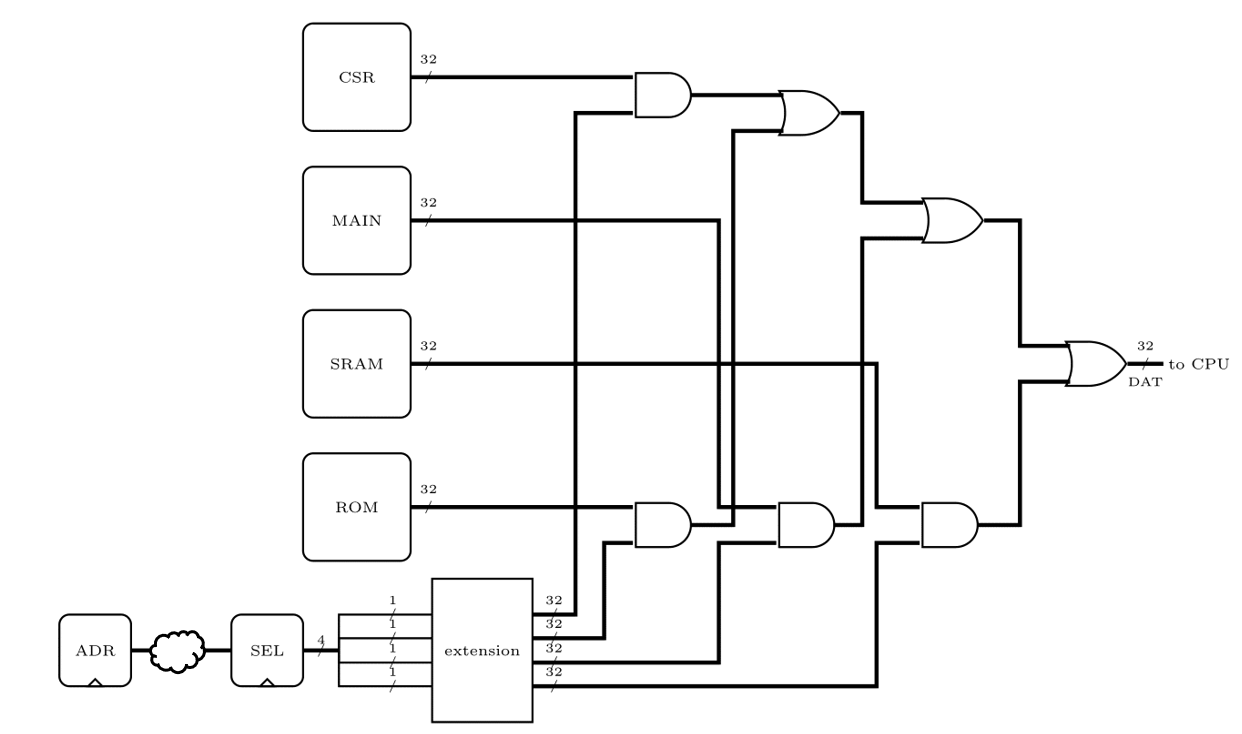
\includegraphics[width=1.1\linewidth]{Chapitre3/figures/sel.png}
  \caption{Connection of selection register with CPU and memory on the bus}
  \label{sel}
\end{figure}

\begin{figure}[t!]
  \centering
  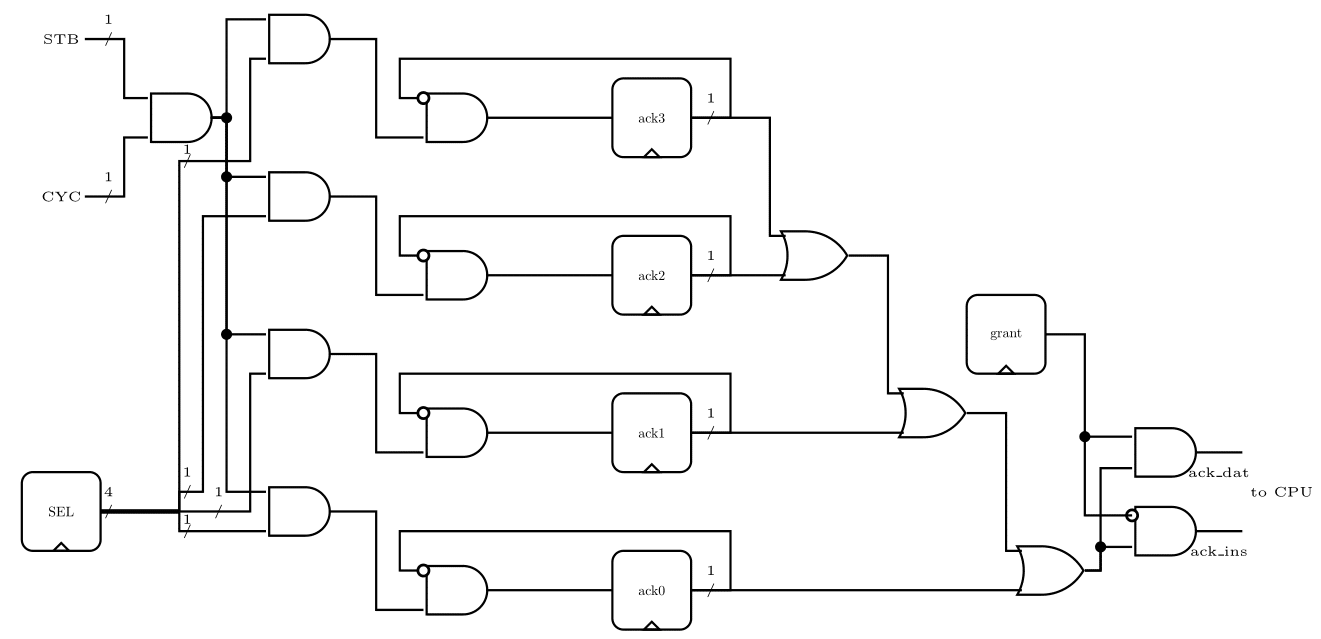
\includegraphics[width=1.1\linewidth]{Chapitre3/figures/ack.png}
  \caption{Connection of acknowledge registers with address registers and memory on the bus}
  \label{ack}
\end{figure}

The Wishbone bus protocol specifies a straightforward, synchronous communication scheme between a single master and one or more slave devices. Figure~\ref{nofault} illustrates the signal behavior during a typical read operation. In systems featuring multiple masters, each transaction begins with an arbitration phase, during which masters must request access to the shared bus. Access is granted via a \texttt{grant} signal issued by the arbiter. In this figure, \texttt{grant} is asserted (\texttt{1}), indicating that the transaction involves data rather than an instruction. This mechanism ensures mutual exclusion by allowing only one master to initiate communication at any given time. In systems with a single master, this arbitration step is bypassed, and the master can initiate a transaction immediately.

Upon receiving bus access, the master asserts \texttt{cyc} (cycle valid) to initiate a valid bus cycle and sets \texttt{stb} (strobe) to indicate a data transfer request. Concurrently, it places the target address on the \texttt{adr} lines and specifies the operation type using the \texttt{we} (write enable) signal: \texttt{we = 1} for a write, and \texttt{we = 0} for a read. In the case of a write, the data is placed on the \texttt{dat\_w} bus (not shown in this figure). These signals collectively define the operation parameters.

The addressed slave monitors the \texttt{cyc} and \texttt{stb} lines. Upon detecting a valid transaction, it responds by asserting \texttt{ack} (acknowledge). In the example shown, \texttt{cyc} and \texttt{stb} are both high, enabling \texttt{ack0}. The acknowledge lines \texttt{ack0} through \texttt{ack3} are OR-combined to form \texttt{ack\_all}, which is selected by the \texttt{grant} signal to produce the data acknowledgment signal \texttt{ACK\_D} and instruction acknowledgment signal \texttt{ACK\_I}. In Figure \ref{architecturebus} we gather these two signals as acknowledgment  signal\texttt{ACK\_I}. This signal confirms the slave has accepted the write or that valid read data is available on \texttt{dat\_r} (labeled \texttt{DAT} in the figure). The \texttt{sel} signal determines which memory block is addressed by the CPU. Here, \texttt{sel = 0010}, indicating that \texttt{dat1} is routed to \texttt{DAT} and forwarded to the CPU cache. Once the master receives \texttt{ACK\_D}, the transaction is complete: for reads, it captures the data on \texttt{dat\_r}; for writes, the operation concludes upon acknowledgment reception. The master may then deassert \texttt{stb} to end the current transfer or \texttt{cyc} to terminate the bus cycle entirely.

After deassertion, the slave releases the \texttt{ack} line, and the bus returns to an idle state. In multi-master environments, the arbiter may now allocate the bus to another requester via the \texttt{grant} mechanism, restarting the communication sequence.

Although this handshake-driven protocol ensures predictable, clock-synchronous communication, it also exposes potential vulnerabilities under fault injection scenarios. For example, if a transient fault prematurely triggers \texttt{ack} or activates \texttt{grant} erroneously, a master may proceed without legitimate access or before the slave is ready. This can lead to data corruption, unintended memory access, or desynchronization between components. Such risks emphasize the importance of protecting arbitration logic and critical control signals in high-assurance systems.

\begin{figure}[t!]
  \centering
  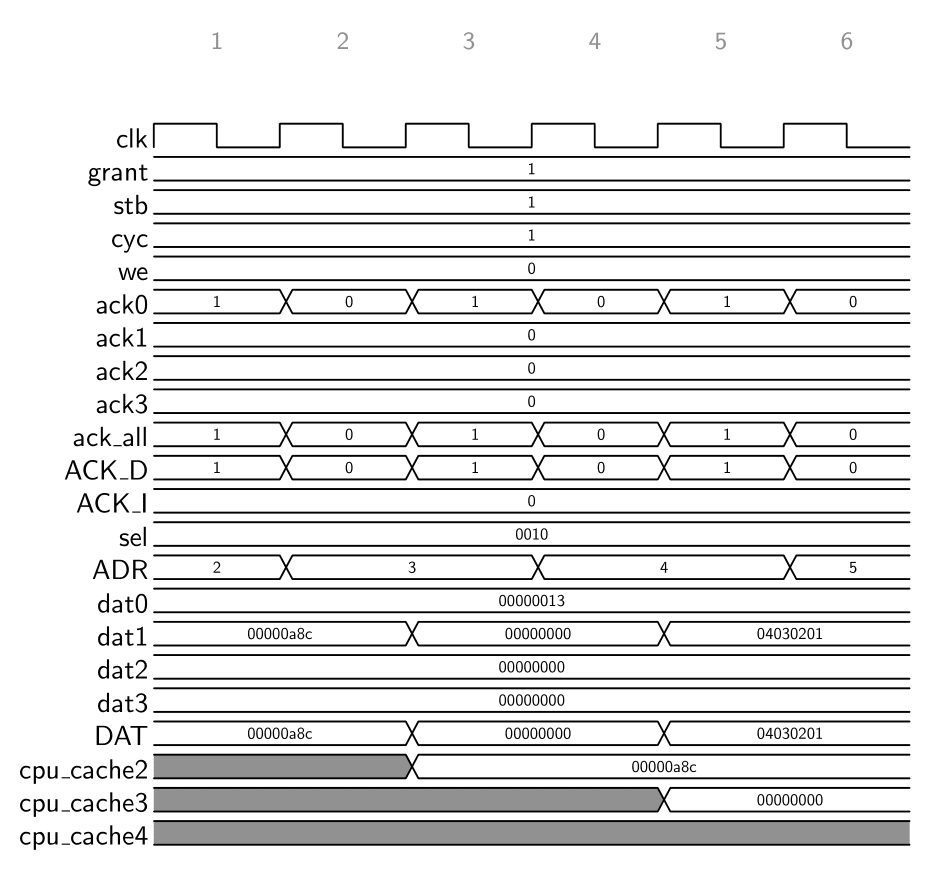
\includegraphics[width=\linewidth]{Chapitre3/figures/nofault.png}
  \caption{Impact of signal transportation without attack in Wishbone}
  \label{nofault}
\end{figure}

\subsection{AXI-Lite}
The AXI-Lite protocol defines a simplified, synchronous communication interface that connects a single master to one or more slave components through a set of well-structured signal channels. This protocol is primarily intended for low-latency, memory-mapped register access within system-on-chip (SoC) architectures, offering a streamlined approach to peripheral communication.

Data exchange in AXI-Lite is orchestrated across five logically independent, unidirectional channels: write address, write data, write response, read address, and read data. Each channel operates using a handshake mechanism built upon two control signals—\texttt{VALID} and \texttt{READY}—that coordinate data transfer. A transaction occurs only when both signals are asserted high, ensuring synchronous and deterministic communication between the master and the slave.

In a write transaction, the master initiates communication by presenting the destination address on the \texttt{AWADDR} signal and setting \texttt{AWVALID} to indicate that the address is ready for sampling. The slave acknowledges its readiness via \texttt{AWREADY}, at which point address transfer is considered complete. Next, the master provides the actual data over the \texttt{WDATA} line, accompanied by the write strobes (\texttt{WSTRB}) that specify active byte lanes, and raises \texttt{WVALID} to signal valid data. The slave asserts \texttt{WREADY} when it is prepared to accept the data. After internal processing, the slave returns a response using the write response channel by asserting \texttt{BVALID} and driving the \texttt{BRESP} signal to indicate the status of the write. The master concludes the transaction by asserting \texttt{BREADY}, acknowledging receipt of the response.

Read transactions follow a similar handshake-based sequence. We present in Figure\ref{axilite}. The master asserts a target read address on \texttt{ARADDR} along with \texttt{ARVALID}, signaling a valid read request. The slave responds with \texttt{ARREADY}, confirming address acceptance. After processing, the slave places the requested data on the \texttt{RDATA} bus (named as \texttt{DAT} in the figure), provides a response code via \texttt{RRESP} (named as \texttt{r\_resp} in the figure), and asserts \texttt{RVALID} (named as \texttt{r\_valid} in the figure) to indicate valid output. The master completes the operation by asserting \texttt{RREADY} (named as \texttt{r\_ready} in the figure), allowing the data and response to be captured.

Each signal in the AXI-Lite protocol has a clearly defined role: address lines (\texttt{AWADDR}, \texttt{ARADDR}) designate the transaction target; data lines (\texttt{WDATA}, \texttt{RDATA}) carry payloads; strobe (\texttt{WSTRB}) selects byte lanes during writes; response signals (\texttt{BRESP}, \texttt{RRESP}) indicate transaction results; and the handshaking signals (\texttt{VALID}, \texttt{READY}) synchronize all transfers without ambiguity. This explicit signal-level orchestration ensures reliable communication, even in timing-constrained environments.

Similar to the Wishbone protocol, the response and selection mechanisms in AXI-Lite govern both the timing and the granularity of data transfers. In standard AXI-Lite implementations, the response signal \texttt{BRESP} is used for write transactions, while \texttt{RRESP} is used for read responses and directly connects to the CPU. However, in the bus architecture generated by LiteX, both \texttt{BRESP} and \texttt{RRESP} are internally mapped to an \texttt{ack} signal, which is subsequently routed to the CPU interface. While the Wishbone protocol explicitly defines \texttt{ACK} and \texttt{SEL} as separate signals, their equivalent functionality in AXI-Lite is implicitly realized through a combination of richer control signals, including \texttt{VALID}, \texttt{READY}, and \texttt{WSTRB}. These signals coordinate transaction sequencing and enable byte-level selection during data transfers, thereby replicating the behavior of traditional acknowledgement and selection lines in a more integrated manner.

\begin{figure}[t!]
  \centering
  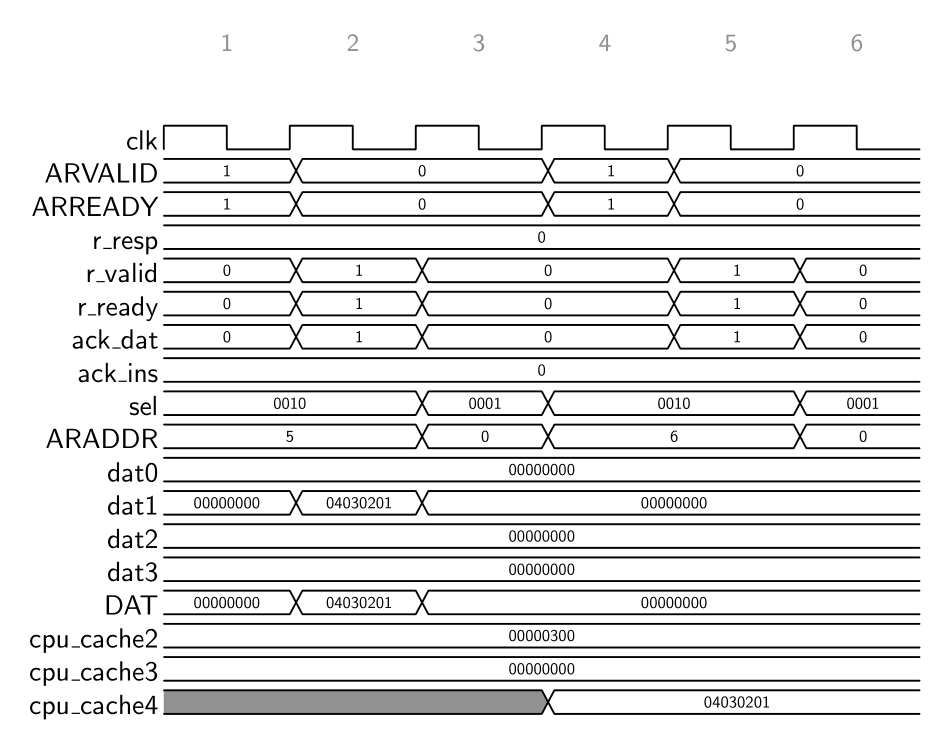
\includegraphics[width=\linewidth]{Chapitre3/figures/axilite.png}
  \caption{Impact of signal transportation without attack in AXI-Lite}
  \label{axilite}
\end{figure}

In addition, we observed that the AXI-Lite bus generated by LiteX introduces a clearing mechanism for improved bus consistency. Specifically, when a particular data channel is active during a read transaction, other unrelated data buses are automatically cleared by setting their values to zero. Furthermore, in the event of a detected fault or error on the bus indicated by state register, read and write data bus is also cleared to zero, and the \texttt{ACK} signal is asserted to indicate that a transaction has been completed, albeit unsuccessfully. This behavior ensures deterministic responses under error conditions and prevents the propagation of invalid data, thereby contributing to system robustness.

Given its predictable behavior and well-defined signaling model, AXI-Lite is particularly suitable for configuration registers, low-bandwidth control paths, and secure interactions between software and hardware components. A thorough understanding of each signal's function within the data transaction phases is essential when implementing or analyzing system interfaces, particularly in contexts such as verification, debugging, or fault injection analysis.

\subsection{AXI}
The AXI (Advanced eXtensible Interface) protocol offers a comprehensive and high-performance interconnect solution within the AMBA specification family. It supports burst-based data transfers, out-of-order transaction handling, and parallel communication from multiple master devices. In contrast, AXI-Lite represents a streamlined variant tailored for low-throughput register-level access, such as configuration or control registers. The two differ significantly in structure and capability. AXI enables multi-beat transfers through parameters like \texttt{AWLEN} and \texttt{AWSIZE}, maintains independent channels for address and data phases, and allows for flexible response ordering. AXI-Lite eliminates these advanced features, restricting all transactions to single-beat operations and reducing the number of control and handshake signals. As a result, AXI-Lite is lightweight, easier to implement, and occupies less silicon area, making it suitable for interfacing with peripheral components. Meanwhile, full AXI is typically used in bandwidth-intensive modules, such as memory subsystems or high-speed I/O. In system-on-chip designs, AXI is often reserved for core interconnects, while AXI-Lite is employed for peripheral configuration paths. Because there are so many features, there are more registers on the AXI.

Similar to the AXI-Lite protocol, the AXI protocol employs response and selection mechanisms to manage the timing and granularity of data transfers. However, in AXI, these mechanisms are significantly more complex and feature-rich. The protocol supports multiple outstanding transactions, burst transfers, and out-of-order responses, requiring a more sophisticated structure for handshaking, address decoding, and response signaling. This added complexity enhances throughput and flexibility but also introduces additional challenges in implementation and verification.

In addition, the AXI interconnect generated by LiteX incorporates a clearing mechanism aligned with AXI-Lite semantics. During a read transaction, when one data channel is actively in use, other unrelated data buses are automatically zeroed out to prevent residual or unintended values. If a fault or error condition is detected—typically flagged by a system state register—the read and write data lines are forcefully cleared to zero. In such cases, the \texttt{ACK} signal is still asserted to mark the end of the transaction, even though it may have failed, thus ensuring protocol completion and preventing bus deadlock.

\section{Vulnerable test on bus}

Following the detailed overview of the Wishbone, AXI-Lite, and AXI bus protocols, the next section focuses on conducting fault injection experiments targeting these three interconnects. By simulating various fault scenarios, we aim to evaluate how each bus architecture responds to disruptive conditions, highlighting their respective resilience and vulnerability. These experiments serve to validate the theoretical analysis presented earlier and provide practical insights for designing more robust countermeasures.

\subsection{Aim}

To systematically assess the inherent robustness of various bus architectures against fault injection, we begin by targeting the Wishbone, AXI-Lite, and AXI buses in their default, unprotected configurations—without any hardware or software countermeasures in place. To eliminate hardware-level protection, we employ the original SoC architecture without added shielding or error-checking logic. To exclude software-level defenses, we use version v0 of the VerifyPin benchmark, which contains no built-in fault detection or recovery mechanisms. This baseline testing phase establishes a neutral, protocol-independent foundation for comparing the fault tolerance characteristics of the three interconnects. All experiments are conducted using consistent fault models and synchronized trigger conditions to ensure fairness and reproducibility. The objective is to observe how transient faults propagate across each bus interface and influence system behavior in the absence of any protective layers. This analysis is essential for exposing the underlying architectural vulnerabilities and for providing a reference point against which the effectiveness of subsequent countermeasure implementations can be measured.

In analyzing successful fault injections across the three bus architectures, we examine several dimensions: the specific registers impacted, the timing windows in which faults are most effective, and whether data or instruction paths are corrupted. While all three buses demonstrate sensitivity to timing-accurate fault injection near transaction boundaries, differences emerge in how and where faults manifest. For example, AXI—with its decoupled read/write channels and handshake signals—shows delayed but wider impact, often corrupting data during burst transfers. In contrast, Wishbone's simpler handshaking and tighter coupling between control and data lead to more localized fault effects, usually within specific instruction or configuration registers. AXI-Lite, being structurally simpler than full AXI but more modular than Wishbone, shows an intermediate pattern. The analysis reveals how bus topology, signal granularity, and transaction sequencing influence the propagation of transient faults and determine the specific functional units affected.

To further differentiate the fault resistance of each bus, we evaluate three experimental metrics: the practical difficulty of injecting effective faults, the overall time required to conduct the campaign, and the number of distinct registers successfully targeted. AXI buses, due to their protocol complexity and the presence of multiple timing domains, typically require more precise injection strategies, increasing the difficulty and experimentation time. However, they also expose a wider attack surface, particularly in burst or pipelined operations. Wishbone, though easier to disrupt due to its predictable signaling and simpler timing, exhibits fewer exploitable registers in a given test case. AXI-Lite lies in between, both in complexity and fault injection difficulty. This comparative study allows us to quantify the attack feasibility for each bus type and prioritize countermeasure deployment based on vulnerability density and ease of exploitation.

\subsection{Step}

We perform the fault injection experiments according to the following procedure. First, we generate the System-on-Chip (SoC) architectures using LiteX, configured as described previously. Specifically, we generate three distinct SoC variants—each using one of the three bus protocols: Wishbone, AXI-Lite, and AXI. These designs maintain consistent CPU and peripheral configurations to ensure fair comparison. Subsequently, the \texttt{VerifyPin} benchmark (version v0), originally written in C, is compiled into a binary file without optimization flags, preserving the instruction-level structure for fault sensitivity.

The resulting binary is then embedded into each SoC variant. Corresponding bitstreams are generated and programmed onto an FPGA development board to validate the correctness of each hardware design under real-world deployment. This hardware verification step ensures that each bus protocol can support basic program execution without protection mechanisms.

In parallel, we initiate a simulation-based workflow using the Verilog source files and memory initialization files generated by LiteX for each SoC. Our first step is to verify that the designs can be successfully compiled and simulated. During this stage, we observe numerous redundant or duplicated signal assignments, particularly in the AXI-Lite and AXI architectures. These redundancies are introduced by LiteX’s automatic code generation process. In the case of AXI-Lite and AXI buses, we encounter compilation errors due to signal redriving, which violate synthesis rules. We address this by manually identifying and removing the redundant statements in an iterative process. Each modification is followed by recompilation to ensure correctness.

Once the designs are successfully compiled, we proceed to simulate all three architectures. Initially, we observe incorrect behavior in program execution. This issue is traced to subtle incompatibilities between the memory layout and the binary. We resolve this by modifying the C source of \texttt{VerifyPin}, recompiling it into a new binary, and converting it again into an initialization file. We then re-integrate this file and verify correct execution through simulation.

To further ensure simulation accuracy and prevent undefined behavior due to uninitialized memory, we explicitly initialize all memory components—except for ROM—with zero values using the assignment \texttt{32'h00000000}. This eliminates the propagation of X-type logic states during simulation, which could otherwise corrupt bus behavior or control signals.

Next, we analyze the internal structure of each SoC to understand how the bus interconnect behaves under normal execution. Using Vivado's elaborated design visualization, we generate detailed RTL schematics for all three designs. These diagrams provide a global overview of the SoC and enable us to classify its components into three functional domains: the CPU core, the bus interconnect, and peripheral memory regions. Based on signal connections and naming conventions, we identify the key registers within each region.

We further categorize all bus-connected registers based on their name, bit-width, and role within the data flow. Registers are grouped into three major types: data-related, address-related, and control-related. This classification allows us to narrow down potential fault injection targets.

After enumerating and analyzing the register set, we exclude certain classes of registers from our attack scope. First, registers storing raw data or memory addresses are ignored, as these can be protected using data integrity mechanisms such as error detection codes or mirrored verification logic between CPU and memory, as discussed in the literature. Secondly, registers controlling the clock and reset logic are also excluded, since clock-glitching attacks on them have already been comprehensively explored. Moreover, since our experiments are conducted entirely within a single SoC instance in simulation, we ignore registers responsible for I/O functions such as LEDs and UART RX/TX interfaces. Finally, we experimentally verify that faulting the Timer-related registers does not affect program control flow in our benchmark, so these are also excluded.

The structure of our attack model is illustrated in Figure~\ref{general}. The figure provides a simplified overview of the SoC’s communication architecture, featuring a central processor and multiple memory-mapped peripheral blocks. Data exchange between the CPU and memory regions—including ROM, RAM, and CSR (which contains the UART and Timer modules)—is conducted via a shared bus. The communication is categorized into three signal domains: data signals (represented in green), address signals (yellow), and control signals (blue). A key control signal, \texttt{SEL}, determines which memory module is accessed during a read or write operation. It achieves this by driving a multiplexer composed of combinational logic. Another crucial signal, \texttt{ACK}, is responsible for handshaking with the CPU to synchronize memory access timing and indicate transaction completion. The precise architecture of these two signal will be presented in next chapter.

\begin{figure}[t!]
  \centering
  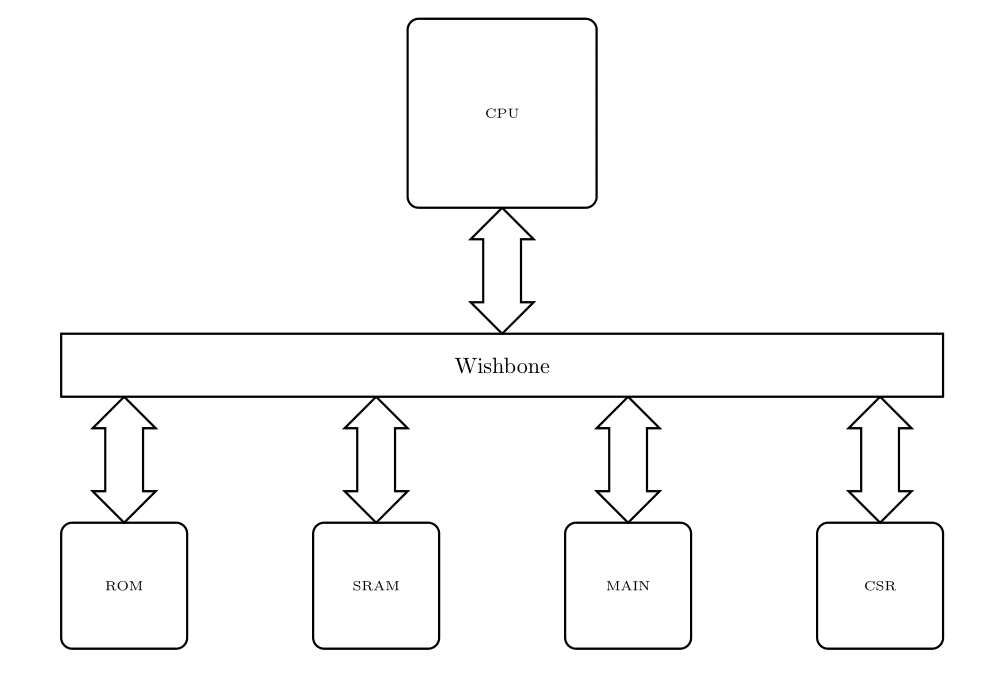
\includegraphics[width=\linewidth]{Chapitre3/figures/general.png}
  \caption{General structure of the SoC and bus}
  \label{general}
\end{figure}

To generate the required simulation scripts, we employ the FISSA tool, which outputs a set of Tcl commands based on the configuration defined in a JSON file. As illustrated in Figure~\ref{conf}, the configuration file \texttt{config\_wop.json} allows users to customize a wide range of parameters to tailor the fault injection campaign.

The parameter \texttt{name\_simulator} specifies the simulation engine in use—such as ModelSim in our case. A group of path-related variables—namely \texttt{path\_tcl\_generation}, \texttt{path\_files\_sim}, \texttt{path\_generated\_sim}, \texttt{path\_results\_sim}, and \texttt{path\_simulation}—are used to define the respective directories: where the FISSA tool is located, where the necessary simulation input files reside, where the generated Tcl scripts are saved, where the simulation results are stored, and where the Verilog-based simulation project is hosted.

The \texttt{threat\_model} field determines the type of attack scenario being used. In our study, four different models are evaluated; the one shown in the figure is the 2-bit-flip attack, denoted in FISSA as \texttt{single\_bitflip\_spatial}. This model simulates spatially localized bit-flip faults. The parameter \texttt{multi\_fault\_injection} governs how many bits are affected in each injection—set to 1 for single-bit faults, and 2 for multi-bit scenarios.

Two additional parameters, \texttt{avoid\_registers} and \texttt{avoid\_log\_registers}, define lists of registers that should be excluded from fault injection or logging, even if they appear in the default target list (\texttt{register.yaml}). In our case, these fields are intentionally left empty since we do not need to exclude any specific registers. Similarly, the parameter \texttt{log\_registers} lists registers that are not part of the original attack list but should still be monitored during simulation. Again, we do not require this feature and thus leave it empty.

The fault injection window is specified by \texttt{fenetre\_tir}, which denotes the range of simulation cycles over which faults will be introduced. This window is calculated by identifying the interval from the point at which the CPU first begins to read the \texttt{code.c} file containing the \texttt{VerifyPIN} function, to the cycle at which the final instruction of that function completes execution. As depicted in the figure, this interval spans from the 20,765th to the 24,037th cycle.

The parameter \texttt{cycle\_ref} indicates the total number of cycles to simulate, starting from the beginning of the attack window. This value is chosen to ensure that the statistical behavior of the system post-injection can be properly observed. Specifically, the simulation must continue long enough to detect whether the variable \texttt{g\_authentifcat}—which reflects the authentication result—transitions to either 0 or 1. A safety margin of several dozen cycles is added beyond the latest occurrence of this event.

The clock period of the SoC, defined by \texttt{cpu\_period}, is set to 8 nanoseconds across all experiments. Finally, the \texttt{batch\_sim} parameter sets the number of individual simulation runs bundled into a single Tcl file. We fix this value at 4000, which allows for a sufficiently large number of simulations per batch while mitigating the risk of simulation crashes due to excessive memory usage.

\begin{lstlisting}[language=json,caption={config.json file},label={conf}]
{
    "name_simulator": "modelsim",
    "path_tcl_generation": "C:/Users/zhao/Desktop/FISSA-main/",
    "path_files_sim": "C:/Users/zhao/Desktop/FISSA-main/simu_files/",
    "path_generated_sim": "C:/Users/zhao/Desktop/FISSA-main/simu_files/generated_simulations/",
    "path_results_sim": "C:/Users/zhao/Desktop/FISSA-main/simu_files/results_simulations/",
    "path_simulation": [
        "C:/Users/zhao/Desktop/mo_project/",
        "__code",
        "/",
        "__code"
    ],
    "threat_model": [
        "single_bitflip_spatial"
    ],

    "multi_fault_injection": 2,
    "avoid_register": [
    ],
    "avoid_log_registers": [
    ],
    "log_registers": [
    ],
    "fenetre_tir": {
        "total": [
            [
                20765,
                24037
            ]
        ]
    },
    "cycle_ref": 3067,
    "cpu_period": 8,
    "batch_sim": {
        "total": 4000
    },
    "name_reg_file_ext_wo_protect": "/faulted-reg.yaml"
}
\end{lstlisting}

The variable \texttt{name\_reg\_file\_ext\_wo\_protect} specifies the path to the register list used for fault injection. This list is defined in a YAML configuration file named \texttt{register.yaml}, which organizes and categorizes the registers targeted during the simulation campaign. A partial excerpt of this file is illustrated in Figure~\ref{yaml} to clarify its structure and contents.

In the file \texttt{register.yaml}, the key \texttt{TOTAL} denotes the name of the overall attack scenario for which the associated registers are configured. Under this heading, each register entry includes the full hierarchical signal name along with the number of bits to be subjected to fault injection. For example, the signal \texttt{sim:/digilent\_tb/UUT/builder\_axirequestcounter0\_full} is marked as a 1-bit register target, indicating that only a single bit within this signal will be perturbed during injection.

It is important to note that every register to be included in the attack must be explicitly listed before the delimiter line represented by \texttt{...}, which signifies the end of the register list. Any register entries placed after this delimiter will not be considered by the FISSA tool during campaign generation. This structure ensures clarity and avoids ambiguity, especially when multiple attack configurations are defined in the same file.

\begin{lstlisting}[language=json,caption={register.yaml file},label={yaml}]
TOTAL:
  -
      name: sim:/digilent_tb/UUT/builder_axirequestcounter0_full
      width: 1
  -
      name: sim:/digilent_tb/UUT/builder_axirequestcounter0_empty
      width: 1
  -
      name: sim:/digilent_tb/UUT/builder_axirequestcounter1_full
      width: 1
  -
      name: sim:/digilent_tb/UUT/builder_axirequestcounter1_empty
      width: 1
  -
      name: sim:/digilent_tb/UUT/builder_basesoc_axi2axilite0_state
      width: 2   
...
\end{lstlisting}

In the file \texttt{code\_execution.py} (see Figure~\ref{code}), we systematically categorize the outcomes of each simulated fault injection campaign. A simulation is considered active when the flag \texttt{sim\_active} equals 1, indicating that a fault was introduced during its execution. From each such instance, we extract several internal state variables to analyze the system behavior:
\begin{itemize}
    \item the program counter (\texttt{value\_pc})
    \item the authentication result flag (\texttt{g\_authenticated})
    \item the crash indicator (\texttt{crash\_flag})
    \item the software detection flag (\texttt{detect\_sw})
    \item the hardware detection flag (\texttt{detect\_hw})
    \item the hardware correction flag (\texttt{correct})
\end{itemize}

Based on the combination of these variables, the simulation outcomes are classified into the following categories:
\begin{itemize}
\item Crash. This outcome corresponds to a scenario in which the system either exceeds the predefined execution timeout or encounters a fatal error. In such cases, the \texttt{crash\_flag} is set to a value other than \texttt{X}, indicating that a crash has occurred. If \texttt{crash\_flag} remains as \texttt{X}, no crash was detected. To determine whether the simulation has timed out, we compute the end time by adding the current cycle count \texttt{cycle\_ref} to the attack injection point. This total is stored in the variable \texttt{now}. If \texttt{now} exceeds a defined threshold (e.g., 24536000ns), the simulation is deemed to have timed out. In either crash scenario, the outcome is recorded with a status value of 1 in \texttt{status\_end}, and \texttt{sim\_active} is reset to its default value of 0 to indicate the end of the fault-injected trial. The cycle at which this occurred is recorded in \texttt{check\_cycle}.

\item Hardware Detection. If the hardware-based fault countermeasure is triggered, it sets the flag \texttt{cm\_d} to 1. This value is assigned to \texttt{detect\_hw}. The detection event is then logged with the value 2 in \texttt{status\_end}.

\item Software Detection. When the software countermeasure is activated, it sets the SRAM-resident variable \texttt{g\_countermeasure} to 1, which is assigned to \texttt{detect\_sw}. In order to ensure this event does not coincide with a correction event, we also verify that \texttt{correct} is equal to 0. This type of software-only detection is logged in \texttt{status\_end} as value 4.

\item Combined Detection and Correction. When both hardware correction and software detection occur simultaneously—i.e., both \texttt{detect\_sw} and \texttt{correct} are 1—the event is logged with the value 3 in \texttt{status\_end}. This indicates that the software mechanism identified the fault, while the hardware mechanism also attempted a correction.

\item Success. This category indicates that the fault successfully bypassed authentication, evidenced by \texttt{g\_authenticated} being set to 1. Within this category, we further distinguish two subcases: If \texttt{correct} equals 1, then the system reached the success state despite the hardware countermeasure having actively corrected an error. This is marked with the value 5 in \texttt{status\_end}. If \texttt{correct} equals 0, then the system reached the success state without any correction having been made, and this is marked with value 6. For the purposes of this study, both subcases are treated as successful attacks. This is because in typical SoC designs, hardware mechanisms that silently correct erroneous data often do not report this activity to the CPU or software layer—they simply propagate the corrected value as though no anomaly occurred.

\item Change. If the injected fault does not lead to a crash, detection, or successful authentication, yet still alters the memory state, it is classified as a change event. These cases indicate latent or silent corruptions. States 7 and 8 in \texttt{status\_end} include both change and silence cases. Further post-simulation memory analysis is required to disambiguate between them.

\item Silence. In this condition, the fault produces no observable effect—no authentication bypass, no detection, and no memory alteration. Like the change case, this state falls under \texttt{status\_end} values 7 and 8. Final classification depends on a deeper inspection of memory integrity and execution traces following the fault event.
\end{itemize}

\begin{lstlisting}[language=python, caption={code\_execution.py}, label={code}]
while {$sim_active == 1} {
    set value_pc [examine -hex /digilent_tb/UUT/VexRiscv/IBusCachedPlugin_fetchPc_pcReg]
    set g_authenticated [string range [lindex [lindex  [examine -hex /digilent_tb/UUT/sram] 0] 4] 10 11]
    set crash_flag [examine -hex /digilent_tb/UUT/VexRiscv/CsrPlugin_exceptionPortCtrl_exceptionContext_code]
    set detect_sw [string range [lindex [lindex  [examine -hex /digilent_tb/UUT/sram] 0] 4] 6 7]
    set detect_hw [examine -hex /digilent_tb/UUT/cm_d]
    set correct [examine -hex /digilent_tb/UUT/cm_c]    
    if {([expr {$crash_flag} != {"4'hx"}]) || ([expr {$now > 24536000} ])} {
        set status_end 1
        set sim_active 0
        set check_cycle [expr [expr $now / 1000 - $start] / $periode] ;
    } elseif {([expr {$detect_hw} == {"1'h1"}])} {
        set status_end 2
        set sim_active 0
        set check_cycle [expr [expr $now / 1000 - $start] / $periode] ;
    } elseif {([expr {$detect_sw} == {"01"}])} {
        if {([expr {$correct} == {"1'h1"}])} {
            set status_end 3
            set sim_active 0
            set check_cycle [expr [expr $now / 1000 - $start] / $periode] ;
        } else {
            set status_end 4
            set sim_active 0
            set check_cycle [expr [expr $now / 1000 - $start] / $periode] ;
        }     
    } elseif {([expr {$g_authenticated} == {"01"}])} {
        if {([expr {$correct} == {"1'h1"}])} {
            set status_end 5
            set sim_active 0
            set check_cycle [expr [expr $now / 1000 - $start] / $periode] ;
        } else {
            set status_end 6
            set sim_active 0
            set check_cycle [expr [expr $now / 1000 - $start] / $periode] ;
        }
    } elseif {([expr {$correct} == {"1'h1"}])} {
        set status_end 7
        set sim_active 0
        set check_cycle [expr [expr $now / 1000 - $start] / $periode] ;
    } else {
        set status_end 8
        set sim_active 0
        set check_cycle [expr [expr $now / 1000 - $start] / $periode] ;
    }
}
\end{lstlisting}

In the \texttt{log.py} function, we define the procedure for recording simulation results. The first instruction, \texttt{set f open \$state\_file a}, initializes the log file by opening it in append mode. The path or filename to this log is stored in the variable \texttt{state\_file}, which ensures that the outcome of each simulation is appended without overwriting prior results.

At the end of each simulation, the system records the final state of several internal variables into this log file. These include:

\begin{itemize}
\item \texttt{cycle\_ref}: the reference cycle count representing the expected number of cycles when the simulation terminates under normal (i.e., non-faulted) conditions.

\item \texttt{check\_cycle}: the actual number of cycles completed in the current simulation run, which may differ from \texttt{cycle\_ref} due to faults, crashes, or early terminations.

\item \texttt{regFilePlugin\_regFile}: the contents of the processor’s register file at the end of the simulation. This reflects the internal CPU state and may reveal corrupted registers or abnormal execution paths.

\item \texttt{sram} and \texttt{main\_ram}: the two primary memory segments of the system. \texttt{sram} typically stores static variables such as flags and counters, while \texttt{main\_ram} holds dynamic execution data and program code.

\item \texttt{storage} and \texttt{storage\_1}: dedicated regions within the CSR (Control and Status Registers) space. These are used to track the operation of countermeasures and other architectural metadata, which can reflect fault detection or correction attempts.

\end{itemize}

By logging the state of these components at the end of every simulation, the framework supports post-execution analysis for identifying the effects of injected faults, including silent data corruptions, unauthorized authentications, or countermeasure activations. This structured output format also facilitates batch comparisons across multiple fault injection trials, enabling statistical summaries and case-by-case investigation.

\begin{lstlisting}[language=python, caption={code\_execution.py}, label={code}]
set f [open $state_file a]
puts $f "\\t\\"simulation_$nb_sim\\": {"

#---- Cycle Checking ----
puts $f "\\t\\t\\"cycle_ref\\": $cycle_ref," 
puts $f "\\t\\t\\"cycle_ending\\": $check_cycle,"

#---- Log Register File ----
for {set j 0} {$j < 32} {incr j} {
    puts $f "\\t\\t\\"RegFilePlugin_regFile/rf$j\\": \\"[examine -hex /digilent_tb/UUT/VexRiscv/RegFilePlugin_regFile\\[{$j}\\]]\\","
}

#---- Log Sram ----
for {set j 0} {$j < 2048} {incr j} {
    puts $f "\\t\\t\\"sram/sr$j\\": \\"[examine -hex /digilent_tb/UUT/sram\\[{$j}\\]]\\","
}

#---- Log Main_ram ----
for {set j 0} {$j < 2048} {incr j} {
    puts $f "\\t\\t\\"main_ram/mr$j\\": \\"[examine -hex /digilent_tb/UUT/main_ram\\[{$j}\\]]\\","
}

#---- Log Storage ----
for {set j 0} {$j < 16} {incr j} {
    puts $f "\\t\\t\\"storage/st$j\\": \\"[examine -hex /digilent_tb/UUT/storage\\[{$j}\\]]\\","
}

#---- Log Storage1 ----
for {set j 0} {$j < 16} {incr j} {
    puts $f "\\t\\t\\"storage_1/st1$j\\": \\"[examine -hex /digilent_tb/UUT/storage_1\\[{$j}\\]]\\","
}
\end{lstlisting}

Due to the large number of generated TCL files, it becomes impractical to execute them manually or manage them individually. To streamline this process, we employ DO files as wrappers to invoke TCL commands. Specifically, we implement a Python function—generatedo.py—to automatically generate a DO file for each corresponding TCL file, ensuring a one-to-one mapping between the two. As shown in Figure~\ref{generatedo}, the script creates 467 DO files, consistent with the total number of TCL scripts produced during the experiment.

The DO files are stored in the same directories as their corresponding TCL files. These directories are grouped according to the four fault injection models, as indicated by the comments in the code (e.g., Bit-Flip, 2 Bit-Flips, Manipulate Register, and Manipulate Two Registers). Each DO file contains a single source path/index.tcl command. This source command instructs the simulator to load and execute the designated TCL script.

By referencing the TCL scripts through these DO files, we significantly simplify batch execution. Instead of invoking individual TCL files manually, we only need to run the associated DO file, which then triggers the corresponding simulation process. This method improves automation, maintains consistency across simulation runs, and reduces the likelihood of human error during the large-scale fault injection campaign.

\begin{lstlisting}[language=python, caption={generatedo.py}, label={generatedo}]
import os
path = "C:/Users/13383/Desktop/FISSA-main/simu_files/generated_simulations/total/total_wop_1_single_bitflip_spatial_2"
# total_wop_1_bitflip_1
# total_wop_1_multi_bitflip_reg_2
# total_wop_1_multi_bitflip_reg_multi_2
# total_wop_1_single_bitflip_spatial_2

n = 467  

for i in range(1, n+1):
    filename = os.path.join(path, f"s{i}.do")
    content = f"source {path}/total_wop_{i}.tcl"
    with open(filename, 'w') as f:
        f.write(content)
\end{lstlisting}

After configuring the Python-based fault injection framework, we executed large-scale simulation campaigns using the generated \texttt{.tcl} command scripts. Specifically, we conducted: 
\begin{itemize}
    \item 94,536 simulation runs on the Wishbone bus,
    \item 1,819,440 runs on the AXI-Lite bus,
    \item 13,385,752 runs on the AXI bus.
\end{itemize}

To support such a large volume of fault injections, simulations were executed on a high-performance server hosting three virtual machines. Each virtual machine was configured with 32~GB of RAM and a 12-core \texttt{x86\_64\_v2\_AES} virtual CPU, backed by an Intel Xeon Gold 5220 processor. This setup enabled parallel processing and efficient resource allocation across the simulation jobs.

The simulation campaign generated over 2~TB of output data, which were stored in structured \texttt{.json} format. To analyze these results, we developed a Python program that parses each \texttt{.json} log and categorizes the outcome of every simulation, based on the final value of the state variable \texttt{status\_end}. This classification is performed for each vulnerability model under all three bus architectures.

The classification logic used in the Python script is as follows figure\ref{analysis}:

If \texttt{status\_end} equals 1, 2, 3, or 4, the script increments the counts corresponding to \textit{Crash}, \textit{Hardware Detection}, \textit{Software Detection \& Hardware Correction}, and \textit{Software Detection}, respectively.

If \texttt{status\_end} equals 5, indicating a hardware-corrected success, the counter for this category is incremented. In addition, metadata such as the fault injection period, register name, register size, and fault location are recorded for later analysis.

If \texttt{status\_end} equals 6, which corresponds to a success without hardware correction, the count for this case is similarly incremented, and related metadata are stored.

If \texttt{status\_end} equals 7 or 8, which refer to either a silent or a memory-change event, a further comparison is performed: For each memory element (e.g., \texttt{sram}, \texttt{main\_ram}), its post-simulation value is compared against the corresponding value in a reference simulation without fault injection. If all memory values match the reference, the case is categorized as \textit{Correct Silence}, and the silence count is incremented. Otherwise, if any difference is observed, the case is classified as a \textit{Change}, and the change counter is increased accordingly.

This automated classification pipeline not only enables large-scale statistical analysis of attack outcomes but also supports fine-grained examination of countermeasure behavior across buses and attack locations. By logging contextual data for each fault instance, we facilitate traceability, reproducibility, and in-depth root cause analysis in the subsequent evaluation chapters. The result of analysis result are reserved in result.json.

\begin{lstlisting}[language=python, caption={analysis.py}, label={analysis}]
if status_end == 1:
    crash += 1
elif status_end == 2:
    detect_hw += 1
elif status_end == 3:
    detect_sw_c += 1
elif status_end == 4:
    detect_sw_n += 1
elif status_end == 5:
    success_c += 1
    if key not in results:
        results[key] = {"cycle_attacked": None, "faulted_register": None, "size_faulted_register": None, "bit_flipped": None}
    results[key]["cycle_attacked"] = value.get("cycle_attacked")
    results[key]["faulted_register"] = value.get("faulted_register")
    results[key]["size_faulted_register"] = value.get("size_faulted_register")
    results[key]["bit_flipped"] = value.get("bit_flipped")    
elif status_end == 6:
    success_n += 1
    if key not in results:
        results[key] = {"cycle_attacked": None, "faulted_register": None, "size_faulted_register": None, "bit_flipped": None}
    results[key]["cycle_attacked"] = value.get("cycle_attacked")
    results[key]["faulted_register"] = value.get("faulted_register")
    results[key]["size_faulted_register"] = value.get("size_faulted_register")
    results[key]["bit_flipped"] = value.get("bit_flipped")                     
elif status_end == 7:
    for subkey in base_data.keys():
        if subkey.startswith('sram/sr') or subkey.startswith('main_ram/mr') or subkey.startswith('storage/st') or subkey.startswith('storage_1/st1'):
            if subkey in data[key]:
                if base_data[subkey] != data[key][subkey]:
                    change += 1
                    silence -= 1
                    key_list.append(key) 
    correct_hw += 1
elif status_end == 8:
    for subkey in base_data.keys():
        if subkey.startswith('sram/sr') or subkey.startswith('main_ram/mr') or subkey.startswith('storage/st') or subkey.startswith('storage_1/st1'):
            if subkey in data[key]:
                if base_data[subkey] != data[key][subkey]:
                    change += 1
                    silence -= 1
                    key_list.append(key)                                                  
    silence += 1
\end{lstlisting}    
\subsection{Analysis}

Since no countermeasures were implemented in our experiments, several system-level responses—such as error detection or recovery mechanisms—were absent. Each simulation outcome was therefore classified into one of the following four categories:

\begin{enumerate}
\item \textbf{Crash:} The simulation terminated abnormally, either due to a timeout or by triggering a fault-induced system crash.
\item \textbf{Success:} The authentication mechanism was bypassed, with the flag \texttt{g\_authenticated} incorrectly set to “1”.
\item \textbf{Change:} The fault altered memory contents, but did not lead to a successful authentication or any crash event.
\item \textbf{Silence:} The injected fault produced no observable effects—no authentication bypass, memory change, or system crash.
\end{enumerate}

We performed extensive fault injection campaigns targeting all three bus protocols—Wishbone, AXI-Lite, and AXI—under multiple fault models. Table~\ref{Vunerabilities on 3 buses} presents a comparative summary of the observed outcomes, detailing the number of occurrences of each result type for every fault model across the different bus architectures. This dataset provides a basis for evaluating the vulnerability profiles of each bus protocol in the absence of defense mechanisms.

\begin{table}
\centering
\caption{Fault injection results for each bus and fault model}
\label{Vunerabilities on 3 buses}
\begin{tabular}{llrrrr}
\toprule
bus & fault model & crash & success & change & slience \\
\midrule
& bitflip & 43 & 24 & 69 & 2438 \\
& manipulate reg   & 288 & 27 & 79 & 6626 \\
& 2 bitflip & 502 & 179 & 479 & 11710 \\
\multirow{-4}{*}{wishbone}  & manipulate 2 regs & 4690 & 515 & 1382 & 65485 \\
\midrule
& bitflip & 282 & 4 & 1913 & 11577 \\
& manipulate reg & 391 & 6 & 2589 & 29942 \\
& 2 bitflip & 10725 & 153 & 69811 & 194831 \\
\multirow{-4}{*}{axi-lite}  & manipulate 2 regs & 36215 & 549 & 224347 & 1236105 \\
\midrule
& bitflip & 158 & 4 & 4833 & 34269 \\
& manipulate reg   & 435 & 6 & 6723 & 90996 \\
& 2 bitflip & 14760 & 333 & 428382 & 1421565 \\
\multirow{-4}{*}{axi} & manipulate 2 regs & 104655 & 1328 & 1514455 & 9762850 \\         
\bottomrule  
\end{tabular}
\end{table}

The total number of executed simulations increases progressively from the Wishbone bus to AXI-Lite and finally to the AXI bus. This trend correlates with the increasing architectural complexity of the bus protocols, as well as the growing number of control and status registers present in more advanced interconnects. As a result, under simple fault models, the Wishbone bus exhibits a relatively higher proportion of successful attacks. This observation suggests that lower-complexity interconnects are more susceptible to basic fault injection techniques, where isolated bit-level disturbances are more likely to produce impactful system disruptions.

To better understand this behavior, we analyzed the injection patterns associated with successful outcomes. A representative case involves the relationship between the \textit{Bit-Flip} model and more complex models such as \textit{2 Bit-Flips} and \textit{Manipulate Two Registers}. For example, if a single-bit corruption in a register (e.g., register \texttt{a}) under the \textit{Bit-Flip} model leads to a successful attack, then a similar outcome may also occur under the \textit{2 Bit-Flips} model—provided one of the two injected faults targets the same bit in \texttt{a}, while the second fault occurs at a location that has no functional impact. In such cases, the success can be attributed solely to the critical bit-flip, and any additional faults are functionally redundant.

Based on this reasoning, we consider that more complex fault models—such as \textit{Manipulate Register}, \textit{2 Bit-Flips}, and \textit{Manipulate Two Registers}—are capable of subsuming the fault conditions of simpler models. In particular, the \textit{Manipulate Two Registers} model inherently encompasses attack scenarios that replicate those found in all prior models. This hierarchical inclusion suggests that evaluating attack models in isolation may obscure the functional overlap among them, and highlights the importance of de-duplicating success cases across fault models when analyzing attack effectiveness.


To accurately estimate the unique number of successful attack cases per model—without double-counting those that are functionally equivalent—we implement a deduplication algorithm in Python, as illustrated in Figure~\ref{newfault}. The methodology is as follows:

Let model \texttt{a} denote a simpler fault model (e.g., \texttt{total\_wop\_1\_bitflip\_1}), and model \texttt{b} denote a more complex one (e.g., \texttt{total\_wop\_1\_single\_bitflip\_spatial\_2}). Both contain a dictionary of successful attack instances parsed from their respective \texttt{.json} result files. Each entry logs metadata including the target register name (\texttt{faulted\_register\_0}, \texttt{faulted\_register\_1}), the bit indices modified (\texttt{bit\_flipped}), and the values injected (\texttt{value\_set}).

We first filter out entries in model \texttt{b} that introduce attacks on registers not present in the trusted vulnerability space—denoted by the list \texttt{valid\_values\_list}. This step ensures that side-effect-free additions to unrelated registers do not disqualify functional equivalence with model \texttt{a}.

Then, for each entry in model \texttt{a}, we iterate through the entries in \texttt{b} and check if any of the following fields match:
\begin{itemize}
    \item the name of at least one faulted register
    \item the bit index that was flipped
    \item the resulting register value post-injection
\end{itemize}

If such conditions are met, the attack in model \texttt{b} is deemed equivalent to one in model \texttt{a}. Otherwise, it is preserved as a distinct entry and stored in the \texttt{invalid\_entries} dictionary.

In this script, we also consider control signals like \texttt{sel}—which indirectly affect the \texttt{ack} signal—as valid fault targets, and therefore include them in \texttt{valid\_values\_list}. The script compares results across models including: \texttt{total\_wop\_1\_bitflip\_1} vs. \texttt{total\_wop\_1\_single\_bitflip\_spatial\_2}, \texttt{total\_wop\_1\_multi\_bitflip\_reg\_2} vs \texttt{total\_wop\_1\_multi\_bitflip\_reg\_multi\_2}.

This de-duplication process is crucial for understanding the actual marginal contribution of each advanced fault model and prevents overestimating their impact due to nested or overlapping attack conditions.

\begin{lstlisting}[language=python, caption={newfault.py}, label={newfault}]
for key, value in b_data['results'].items():
    if key.startswith('simulation'):

        faulted_reg_0_in_list = value.get('faulted_register_0') in valid_values_list
        faulted_reg_1_in_list = value.get('faulted_register_1') in valid_values_list
        
        cycle_attacked = value.get('cycle_attacked')
        is_cycle_and_faulted_registers_matched = False
        
        for a_key, a_value in a_simulation_data.items():
            if a_value['cycle_attacked'] == cycle_attacked:
                if ((value.get('faulted_register_0') == a_value['faulted_register'] and value.get('bit_flipped_0') == a_value['bit_flipped'] and value.get('value_set_0') == a_value['value_set']) or
                    (value.get('faulted_register_1') == a_value['faulted_register'] and value.get('bit_flipped_1') == a_value['bit_flipped'] and value.get('value_set_1') == a_value['value_set'])):
                    is_cycle_and_faulted_registers_matched = True
                    a_value['correspond_time'] = a_value['correspond_time'] + 1 
                    break
        
        if not (faulted_reg_0_in_list and faulted_reg_1_in_list) and not is_cycle_and_faulted_registers_matched:
            invalid_entries[key] = value

newfault_file_path = os.path.join(b_folder, 'newfault.json')
with open(newfault_file_path, 'w') as newfault_file:
    json.dump(invalid_entries, newfault_file, indent=4)
    json.dump(a_simulation_data, newfault_file, indent=4)
print(f"Invalid faults saved to {newfault_file_path}")

valid_values_list = ['sim:/digilent_tb/UUT/builder_basesoc_state', 'sim:/digilent_tb/UUT/builder_slave_sel_r', 'sim:/digilent_tb/UUT/main_basesoc_interface0_ram_bus_ack', 'sim:/digilent_tb/UUT/main_basesoc_interface1_ram_bus_ack', 'sim:/digilent_tb/UUT/main_basesoc_ram_bus_ack']
a_folder = f"D:/{bench_name}/{model_name}/total_wop_1_bitflip_1"
b_folder = f"D:/{bench_name}/{model_name}/total_wop_1_single_bitflip_spatial_2"
check_analysis_json(a_folder, b_folder, valid_values_list)

a_folder = f"D:/{bench_name}/{model_name}/total_wop_1_multi_bitflip_reg_2"
b_folder = f"D:/{bench_name}/{model_name}/total_wop_1_multi_bitflip_reg_multi_2"
check_analysis_json(a_folder, b_folder, valid_values_list)
\end{lstlisting}   

Using the deduplication program described above, we are able to systematically count, for each successful case under the \textit{Manipulate Two Registers} fault model, the following critical attributes: the names of the registers targeted by the attack, the specific effect or outcome resulting from the fault injection (e.g., authentication bypass, silent corruption), the cycle period in which the attack occurred, whether the fault targeted instruction memory or data memory, the number of times each unique fault scenario occurred, and whether the same outcome had already appeared in simpler models such as \textit{Bit-Flip}, \textit{2 Bit-Flips}, or \textit{Manipulate Register}.

These factors were deliberately selected to support a multifaceted understanding of the behavior and severity of fault injections in a System-on-Chip (SoC) environment. Identifying the specific registers involved in a successful fault is fundamental to vulnerability localization. Registers such as configuration flags, program counters, or authentication variables may represent high-value targets whose compromise leads to critical security violations. By collecting these names, we can construct a register vulnerability profile and assess which parts of the system are inherently more susceptible to low-level perturbations.

Not all successful faults are equally severe. Some may simply cause non-functional side effects, while others result in functional compromise such as bypassing security checks. Logging the effect of each attack helps prioritize vulnerabilities, especially in distinguishing between critical integrity violations (e.g., setting \texttt{g\_authenticated} to 1) and benign disruptions (e.g., register corruption without propagation).

The timing of an injected fault is often as critical as its location. Certain execution windows—such as just before a conditional branch or during memory load operations—are particularly sensitive to disruption. Recording the fault injection cycle allows us to identify time-dependent vulnerabilities and can inform the design of temporal countermeasures such as redundancy or instruction duplication.

Whether the fault targets instruction memory or data memory can have a profound impact on system behavior. Attacks on instruction memory may induce control-flow hijacking or invalid opcode execution, while faults in data memory may lead to incorrect variables or silent corruption. Separating these cases aids in understanding the attack surface and selecting appropriate protection schemes (e.g., ECC for data, checksum or signatures for code).

By aggregating how many times a specific fault condition leads to a successful outcome, we can quantify its statistical significance. Some attacks may appear successful due to randomness or rare coincidences, while others may succeed systematically across a wide range of runs. This statistical insight allows us to differentiate between unstable, environment-specific effects and repeatable, architecture-driven weaknesses.

Finally, comparing each successful case against the outcomes of simpler models allows us to identify whether a complex fault model (such as \textit{Manipulate Two Registers}) contributes any unique successful cases not covered by the simpler models. This distinction is essential for understanding the marginal power of more complex attacks and for avoiding overestimation in vulnerability reporting. If a complex attack only reproduces what simpler models can already achieve, its actual impact on security posture may be limited.

The table is shown below Tab\ref{result on Wishbone}\ref{result on AXI-Lite}\ref{result on AXI}, for which a detailed analysis follows.

\begin{table}[htbp] 
\centering
\caption{Fault injection results for Wishbone bus} 
\label{result on Wishbone} 
\resizebox{\textwidth}{!}{%
\begin{tabular}{llllll} 
\toprule
vunerable reg & attack effect & \multicolumn{1}{l}{attack moment} & influence data & \multicolumn{1}{l}{fault number} & already present in \\
\midrule 
ack reg not in use & delay/advance signal in bus & 10142 & if(byteArrayCompare == \textcolor{red}{1}) & 51 & Bit-flip \\
ack reg in use & delay/advance signal in bus & 10158 & if(byteArrayCompare == \textcolor{red}{1}) & 16 & Bit-flip \\
ack reg not in use & delay/advance signal in bus & 10158 & \textcolor{red}{if}(byteArrayCompare == 1) & 54 & Bit-flip \\
ack reg in use & delay/advance signal in bus & 10174 & \textcolor{red}{if}(byteArrayCompare == 1) & 19 & Bit-flip \\
ack reg in use & delay/advance signal in bus & 10590 & return \textcolor{red}{0} & 19 & Bit-flip \\
ack reg not in use & delay/advance signal in bus & 10654 & i \textless \textcolor{red}{size} & 75 & Bit-flip \\ 
ack reg in use & delay/advance signal in bus & 10670 & i \textless \textcolor{red}{size} & 16 & Bit-flip \\
ack reg not in use & delay/advance signal in bus & 10670 & i \textless \textcolor{red}{size} & 54 & Bit-flip \\
ack reg not in use & delay/advance signal in bus & 10750 & size value & 75 & Bit-flip \\ 
ack reg not in use & delay/advance signal in bus & 10766 & address of card pin & 54 & Bit-flip \\ 
ack reg in use & delay/advance signal in bus & 10766 & size value & 16 & Bit-flip \\
sel reg & influence sel directly & 10774 & size value & 16 & Bit-flip \\
sel reg & influence sel directly & 10774 & size value & 32 & Manipulate Register \\
ack reg not in use and builder\_grant & delay/advance signal in bus & 10742 & size value & 3 & 2 Bit-Flips \\
ack reg not in use and ack reg in use & delay/advance signal in bus & 10758 & size value & 3 & 2 Bit-Flips \\
ack reg not in use and ack reg in use & delay/advance signal in bus & 10150 & if(byteArrayCompare == \textcolor{red}{1}) & 3 & 2 Bit-Flips \\ 
ack reg not in use and ack reg in use & delay/advance signal in bus & 10166 & \textcolor{red}{if}(byteArrayCompare == 1) & 3 & 2 Bit-Flips \\
ack reg not in use and ack reg in use & delay/advance signal in bus & 10582 & return \textcolor{red}{0} & 3 & 2 Bit-Flips \\ 
ack reg not in use and ack reg in use & delay/advance signal in bus & 10662 & i \textless \textcolor{red}{size} & 3 & 2 Bit-Flips \\ 
\bottomrule 
\end{tabular} 
}
\end{table}


\begin{table}
\caption{Fault injection results for AXI-Lite}
\label{result on AXI-Lite}
\resizebox{\textwidth}{!}{%
\begin{tabular}{llllll}
\toprule
vunerable reg & attack effect & \multicolumn{1}{l}{attack moment} & influence data & \multicolumn{1}{l}{fault number} & already present in \\
\midrule
state & delay/advance signal in bus, reset data, influence sel & 18790 & card pin & 91 & Bit-flip \\
state & delay/advance signal in bus, reset data, influence sel & 18790 & card pin & 91 & Bit-flip \\
state & delay/advance signal in bus, reset data, influence sel & 18798 & card pin & 92 & Bit-flip \\
state & delay/advance signal in bus, reset data, influence sel & 18806 & card pin & 80 & Bit-flip \\
state & delay/advance signal in bus, reset data, influence sel & 18798 & card pin & 89 & Bit-flip \\
state & influence sel to read reseted rom & 18798 & card pin & 87 & Manipulate Register \\
state & delay/advance signal in bus, reset data, influence sel & 18790 & card pin & 89 & Manipulate Register \\
state & delay/advance signal in bus, influence sel to read reseted sram & 18790 & card pin & 1 & 2 Bit-Flips \\
sel and state & influence sel to read sram+rom & 19326 & assign size \textcolor{red}{4} & 1 & 2 Bit-Flips \\
sel and state & influence sel to read sram+rom & 19862 & if (i\textless{}\textcolor{red}{size}) & 1 & 2 Bit-Flips \\
state & influence sel, reset data & 18790 & card pin & 1 & 2 Bit-Flips \\
state & delay/advance signal in bus, reset data, influence sel & 18774 & card pin & 1 & 2 Bit-Flips \\
state and done & delay/advance signal in bus, influence sel to read reseted rom & 18790 & card pin & 1 & 2 Bit-Flips \\
state & delay/advance signal in bus & 19030 & if(function = \textcolor{red}{1}) & 1 & 2 Bit-Flips \\
state & delay/advance signal in bus & 19054 & \textcolor{red}{if}(function = 1) & 1 & 2 Bit-Flips \\
state & delay/advance signal in bus & 19286 & assign size \textcolor{red}{4} & 1 & 2 Bit-Flips \\
state & delay/advance signal in bus & 19310 & assign size \textcolor{red}{4} & 1 & 2 Bit-Flips \\
state & delay/advance signal in bus & 19726 & \textbf{return \textcolor{red}{0}} & 1 & 2 Bit-Flips \\
state & delay/advance signal in bus & 19750 & \textbf{\textcolor{red}{return 0}} & 1 & 2 Bit-Flips \\
state & delay/advance signal in bus & 19846 & i \textless \textcolor{red}{size} & 1 & 2 Bit-Flips \\
state & delay/advance signal in bus, reset data, influence sel & 18774 & card pin & 1 &  \\
state & delay/advance signal in bus, reset data, influence sel & 18766 & card pin & 1 &  \\
sel and state & influence sel to read sram+rom+main\_ram & 19326 & assign size \textcolor{red}{4} & 1 &  \\
sel and state & influence sel to read sram+rom+main\_ram & 19862 & if (i\textless{}\textcolor{red}{size}) & 1 &  \\
sel and state & influence sel to read sram+rom+csr & 19326 & assign size \textcolor{red}{4} & 1 &  \\
sel and state & influence sel to read sram+rom+csr & 19862 & if (i\textless{}\textcolor{red}{size}) & 1 &  \\
sel and state & influence sel to read sram+rom+main\_ram+csr & 19326 & assign size \textcolor{red}{4} & 1 &  \\
sel and state & influence sel to read sram+rom+main\_ram+csr & 19862 & if (i\textless{}\textcolor{red}{size}) & 1 & \\
\bottomrule
\end{tabular}
}
\end{table}

\begin{table}
\caption{Fault injection results for AXI bus}
\label{result on AXI}
\resizebox{\textwidth}{!}{%
\begin{tabular}{llllll}
\toprule
vunerable reg & attack effect & \multicolumn{1}{l}{attack moment} & influence data & \multicolumn{1}{l}{fault number} & already present in \\
\midrule 
done & delay/advance signal in bus, read reseted sram, influence sel & 21453 & card pin & 223 & Bit-flip \\
state & delay/advance signal in bus, reset data, influence sel & 21469 & card pin & 212 & Bit-flip \\
state & delay/advance signal in bus, read reseted sram, influence sel & 21453 & card pin & 223 & Bit-flip \\
state & delay/advance signal in bus, reset data, influence sel & 21469 & card pin & 212 & Bit-flip \\
state & delay/advance signal in bus, reset data, influence sel & 21453 & card pin & 222 & Bit-flip \\
state & delay/advance signal in bus, influence sel to read reseted sram & 21445 & card pin & 223 & Bit-flip \\
state & influence sel to read reseted rom & 21453 & card pin & 224 & Manipulate Register \\
state & delay/advance signal in bus, reset data, influence sel & 21445 & card pin & 223 & Manipulate Register \\
state and done & delay/advance signal in bus, influence sel to read reseted rom & 21445 & card pin & 1 & 2 Bit-Flips \\
\bottomrule 
\end{tabular}
}
\end{table}

A preliminary analysis of the results table reveals several noteworthy trends. In the Wishbone architecture, the vast majority of successful fault injections originate from the \textit{Bit-Flip} model. In contrast, the \textit{Manipulate Register} and \textit{2 Bit-Flips} models contribute only a small fraction of successful cases, and no unique successful attacks are observed from the \textit{Manipulate Two Registers} model. Interestingly, the majority of effective faults target the \texttt{ack} signal, whose manipulation results in protocol desynchronization. Most of these attacks lead to effects resembling clock glitching—such as delayed or prematurely asserted control signals—rather than direct logic corruption. Furthermore, the majority of successful faults under Wishbone are observed to target instructions, likely due to the protocol’s simpler scheduling mechanism and limited protection over the instruction flow path.

In the case of AXI-Lite, both the \textit{Bit-Flip} and \textit{Manipulate Register} models account for the majority of successful cases, indicating that single-point and targeted register faults remain effective despite the slightly more complex bus structure. The \textit{2 Bit-Flips} and \textit{Manipulate Two Registers} models, again, contribute marginally, with very few or no distinct successes beyond what simpler models have already achieved. Successful attacks in AXI-Lite tend to focus on the \texttt{STATE} signal, whose alteration can stall or prematurely transition finite-state machines governing transaction phases. The effects of these faults continue to resemble temporal misalignments—delay or advance of bus-level handshakes—and are often indistinguishable from those induced by physical glitches. Notably, in AXI-Lite, successful fault locations are nearly evenly split between instruction and data paths, reflecting a wider fault surface compared to Wishbone.

In the full AXI implementation, the trend remains broadly consistent. The \textit{Bit-Flip} and \textit{Manipulate Register} models dominate the space of successful injections, while the \textit{2 Bit-Flips} model contributes very few new outcomes, and the \textit{Manipulate Two Registers} model fails to produce any uniquely successful cases. Most successful attacks target the \texttt{STATE} signal, similar to AXI-Lite, although a noticeable portion also exploit the \texttt{DONE} signal, which signifies transaction completion. The fault effects predominantly manifest as timing violations on protocol-level signals—again echoing characteristics of clock glitches—causing premature or delayed bus responses. Unlike Wishbone and AXI-Lite, in AXI, nearly all successful faults affect data transfers rather than instructions, possibly due to AXI’s decoupled read/write channels and more complex buffering, which offer more timing windows for perturbation during data movement.

Taken together, these observations suggest that while more sophisticated fault models (e.g., 2-bit or multi-register manipulations) theoretically offer a wider attack surface, they rarely produce new, effective outcomes in practice under simple fault scenarios. Single-bit faults remain highly effective, especially when strategically located on control signals critical to bus sequencing. Moreover, attacks that produce glitch-like effects—whether via physical fault injection or software-level emulation—are often sufficient to induce exploitable behavior even in more complex bus architectures.

A closer examination of successful cases reveals two dominant mechanisms: manipulation of the \texttt{ACK} signal, which alters the timing of data retrieval, and corruption of the \texttt{SEL} signal, which changes the targeted memory block. These effects can manifest independently or concurrently. When both signals are impacted in a single injection, their interactions can be either cooperative or overriding. Since all the attacks attack the ACK signal or SEL signal at the root cause, we would like to understand the specifics further. Attacks Based on Table \ref{result on Wishbone} \ref{result on AXI-Lite} \ref{result on AXI}, whether the target register was affected by the ACK signal or SEL signal under each attack, and the number of times each attack was performed, we calculated the percentage of attacks that were successful due to the ACK or SEL signal being affected. In Table~\ref{Percentage on 3 buses}, we report the relative occurrence of each mechanism under the "Manipulate Two Registers" fault model. If both signal types are affected simultaneously, each is counted as half an instance; if one effect dominates, the suppressed one is excluded from the count.

The root cause of these vulnerabilities can be traced to architectural design. In the VexRiscv CPU, the \texttt{ACK} signal directly governs data transfers, yet no timing violation detection is embedded at the bus level. Conversely, the \texttt{SEL} signal is used to select among four memory blocks via combinational logic, allowing an attacker to redirect data access arbitrarily if this signal is compromised.

Empirical results also show that \texttt{ACK}-related attacks are more prevalent than those targeting \texttt{SEL}. On the Wishbone bus, the \texttt{ACK} signal is register-based and represented by a 4-bit value; flipping any of these bits can disrupt data transfer, increasing the attack surface and success probability. In AXI-Lite and AXI, fault injection targeting status registers can inadvertently enable the error correction path, setting the read-valid signal to inactive and forcing \texttt{ACK} to remain asserted—thus emulating a successful read cycle. Since the status register has multiple entry points for perturbation, the success rate remains non-trivial.

In contrast, \texttt{SEL}-based attacks are more constrained. Their effectiveness is heavily influenced by memory initialization states, memory layout strategies, and the behavior defined by the underlying assembly code. Notably, on the AXI bus, altering the \texttt{SEL} signal requires the coordinated corruption of three registers within a single injection event—rendering the success rate of the "Manipulate Two Registers" model effectively zero.

\begin{table}
\caption{Percentage of affected signals by type under successful manipulate 2 regs attacks across three bus architectures}
\label{Percentage on 3 buses}
\begin{tabular}{llrr}
& wishbone & axi-lite & axi \\
ack relate & 90.39\% & 82.51\% & 74.70\% \\
sel relate & 9.61\% & 17.49\% & 25.30\% \\
\end{tabular}
\end{table}

Table~\ref{Percentage data} presents the proportion of instruction-related and data-related vulnerabilities observed under the “Manipulate Two Registers” fault model across the three evaluated bus protocols.

On the Wishbone bus, a high proportion of the observed faults affect instruction execution. This trend is primarily attributed to the frequent corruption of control-flow-relevant instructions such as \texttt{lui} and \texttt{mv}, which are commonly used for register initialization and data movement. These instructions, when corrupted, can easily disrupt the program’s control flow or cause unintended memory access, leading to successful attacks. The relatively simple structure of the Wishbone bus makes these control-flow instructions particularly exposed, thus elevating the overall ratio of instruction-related faults.

In contrast, the AXI-Lite and AXI buses exhibit a different pattern, with data-related vulnerabilities becoming more prevalent. This shift is closely linked to the lightweight error-handling behavior embedded in the LiteX-generated bus structures. Specifically, when faults target control or status registers associated with data handling, the system may respond by resetting corrupted values to zero. In our benchmark configuration, the default user PIN is initialized to “0000.” Therefore, fault-induced zeroing of the card PIN register may cause it to match the legitimate user PIN, effectively bypassing authentication. Under such conditions, unauthorized access is achieved not by altering control instructions, but by unintentionally aligning sensitive data through register corruption.

This contrast highlights the protocol-dependent nature of fault effects: while instruction corruption dominates on simpler buses, data corruption becomes the primary vector for successful exploitation on more complex buses that feature basic fault-containment logic.

\begin{table}
\caption{Percentage of data or instruction read by manipulate 2 regs attacks across three bus architectures}
\label{Percentage data}
\begin{tabular}{llrr}
\toprule
& wishbone & axi-lite & axi \\
\midrule
ack relate & 28.16\% & 97.27\% & 100\% \\
sel relate & 9.32\% & 2.73\% & 0\% \\
\bottomrule
\end{tabular}
\end{table}


Additionally, across all three bus protocols, we observed that fault effects for all four injection models consistently occurred during CPU data read phases. This pattern is attributed to the structure of the \texttt{VerifyPin} benchmark, which includes very few write operations. Moreover, the registers responsible for handling write transactions on each bus are limited in number and infrequently accessed, making them less exposed to injection and thus reducing the likelihood of write-related fault effects.

Based on our experimental observations in Table\ref{result on Wishbone} \ref{result on AXI-Lite} \ref{result on AXI}, we categorized the possible fault-induced behaviors for each attack model across the three bus types into the following classes. 

\begin{itemize}
\item \textbf{Instruction skip:} The CPU skips execution of the next instruction or bypasses the corresponding data fetch.
\item \textbf{Data reset:} The affected instruction or data is replaced by its default (typically zero) value.
\item \textbf{Data misread:} The CPU reads data from an incorrect address location.
\item \textbf{Data multiread:} The CPU erroneously fetches data from multiple locations, leading to inconsistent or unintended values.
\end{itemize}

These classifications serve as a basis for identifying common fault manifestations and evaluating their severity across different bus protocols. Note that the above fault-behavior-models can be transformed into each other under certain conditions. For example, if the instruction or data reset has no additional effect, then data reset can be regarded as instruction skip, and if the data read by the fault is 0, then data multiread can be regarded as data reset.

We summarize the possible performances of each bus under each attack in the table {compare bus} based on experimental results and theoretical calculations. From the table, it can be seen that attacking the wishbone bus produces the richest results, followed by AXI-lite, and the least by AXI. this is because the AXI bus has a more complex structure, which makes it harder for an attack to be successful with fewer fault effects. Also an attack effect can be explained as multiple fault-behavior-models. This is because the fault-behavior-models can be transformed as we talk before. Also in real attack, a fault will not only propagate in one single path. 

\begin{table}[]
\caption{Possible fault exploration for different buses}
\label{compare bus}
\begin{tabular}{llll}
\toprule
                                          & wishbone         & axi-lite         & axi          \\
\multirow{3}{*}{Bit-flip}                 & instruction skip & data reset       & data reset   \\
                                          & data reset       &                  & data misread \\
                                          & data multiread   &                  &              \\
\midrule                                          
\multirow{4}{*}{Manipulate Register}      & instruction skip & data reset       & data reset   \\
                                          & data reset       & data misread     & data misread \\
                                          & data misread     &                  &              \\
                                          & data multiread   &                  &              \\
\midrule                                          
\multirow{4}{*}{2 Bit-Flips}              & instruction skip & instruction skip & data reset   \\
                                          & data reset       & data reset       & data misread \\
                                          & data misread     & data misread     &              \\
                                          & data multiread   & data multiread   &              \\
\midrule
\multirow{4}{*}{Manipulate Two Registers} & instruction skip & data reset       & data reset   \\
                                          & data reset       & instruction skip & data misread \\
                                          & data misread     & data misread     &              \\
                                          & data multiread   & data multiread   &             \\
\bottomrule                         
\end{tabular}
\end{table}

\section{Conclusion}
In this chapter, we examined the process and implications of conducting vulnerability assessments on different bus protocols, focusing particularly on the methodology (aim, steps, and analysis) of fault injection experiments. The results provide valuable insights for system designers selecting a bus protocol when constructing secure SoCs.

First, based on our observations across various fault models and bus architectures, we propose several recommendations for practitioners:

\begin{itemize}
\item \textbf{Prioritize protection of control registers:} Designers should implement reinforced protection mechanisms around data path control elements such as handshake and state registers. While advanced bus protocols offer inherent resistance due to their layered design, they typically involve a larger number of internal control registers. This complexity opens avenues for advanced or cumulative fault injection approaches that may bypass basic protections.

\item \textbf{Reinforce handshake response logic:} Fault injection targeting handshake mechanisms (such as the \texttt{ACK} signal) often triggers instruction skipping, even under simple injection models. Similarly, attacks on chip-select signals (e.g., \texttt{SEL}) frequently cause erroneous memory access. Due to the relatively low effort required to manipulate these components, handshake-related logic should be treated as a high-risk area warranting dedicated countermeasures.

\item \textbf{Go beyond traditional error handling:} Conventional error recovery mechanisms may prove inadequate under adversarial fault injection scenarios. Designers should reassess fault tolerance strategies with a threat-oriented perspective, focusing on limiting fault propagation within the data flow. This includes isolating error-handling logic from critical data paths and reducing reliance on global reset or recovery signals that may themselves be fault targets.

\item \textbf{Mitigate effects of zero-value initialization:} Faults that force registers or memory fields to zero—especially during critical execution stages—can severely compromise system integrity. To counter this, security-critical variables (e.g., cryptographic keys, authentication tokens) should be protected via masking, write-once protections, or runtime validation. Systems should also be capable of detecting anomalous all-zero patterns as a form of fault detection or input sanitization.
\end{itemize}

Our empirical findings reveal that the Wishbone bus, due to its structural simplicity and minimalistic protocol design, is particularly susceptible to fault injection attacks—especially those affecting instruction flow and register behavior. This vulnerability, while posing a challenge, also presents an opportunity: the predictable behavior of the Wishbone bus under attack enables clearer classification of fault effects, making it a suitable candidate for developing and validating fault detection and mitigation strategies.

In contrast, AXI and AXI-Lite buses possess a significantly larger register footprint and intricate control logic. While this complexity can obscure certain low-level attacks, it also introduces a broader attack surface. The sheer number of possible injection points complicates systematic testing and slows down the iteration of countermeasure design. As a result, comprehensive testing on these buses would require extended timeframes—often several months—rendering them less practical for rapid experimentation.

Given these trade-offs, our research narrows its focus to the Wishbone bus as a controllable and transparent testbed for investigating countermeasures against fault injection. Its reduced architectural complexity allows for high-precision experimentation, clearer failure attribution, and more reliable evaluation of security enhancements.

In the following chapter, we present a detailed analysis of hardware and software countermeasures tailored for the Wishbone protocol. We compare existing solutions, discuss their trade-offs, and introduce our own proposed mitigation strategy—designed to balance overhead, effectiveness, and ease of integration within a typical SoC design flow.